\chapter{System Design}

This section is based on the final product of the project. Any compatibility or deployment issues that have been mentioned will be discussed in the system evaluation section.

\section{CI/CD Design and Implementation}
GitHub Actions is used as the CI/CD tool in this project. Workflow files (.yml or .yaml) that automate tests, deployment, etc. are assigned using GitHub Actions. It is possible to run the workflow automatically after certain GitHub events like commit push. A green tick or a red cross will be shown beside the commit in the repository to indicate if the workflow has been completed successfully.

Workflow files can be designed manually or by using recommended workflows on GitHub such as Jekyll or readily made template like JupyterLite. In this project, the pipeline is designed manually. The workflow is set up at the start of the project alongside with the coding environment. The testing and the deployment part of the workflow is designed after the website is fully working. Redirect to the GitHub repository page \href{https://github.com/gabhang/final-year-project}{here} to access the workflow file.

Figure~\ref{image:full-workflow} shows the yml file of the workflow. The workflow is triggered whenever a commit is pushed to the main branch. The workflow has one job named "build" that will run on an Ubuntu operating system that has five steps. 

\begin{enumerate}
  \item Checkout from the repository for automation.
  \item Setup Node.js version 18.x.
  \item Install dependencies using npm
  \item Run tests using npm with designed test suite integrated in the project with \texttt{npm install} command.
  \item Deploy the code to Heroku using the \textit{akhileshns/heroku-deploy} action with the Heroku API key the app name and the email of the account. The Heroku API key is stored in GitHub secrets and is accessed through the \$\{\{ secrets.HEROKU\textunderscore API\textunderscore KEY \}\} variable.
\end{enumerate}

\begin{figure}[h!]
    \centering
    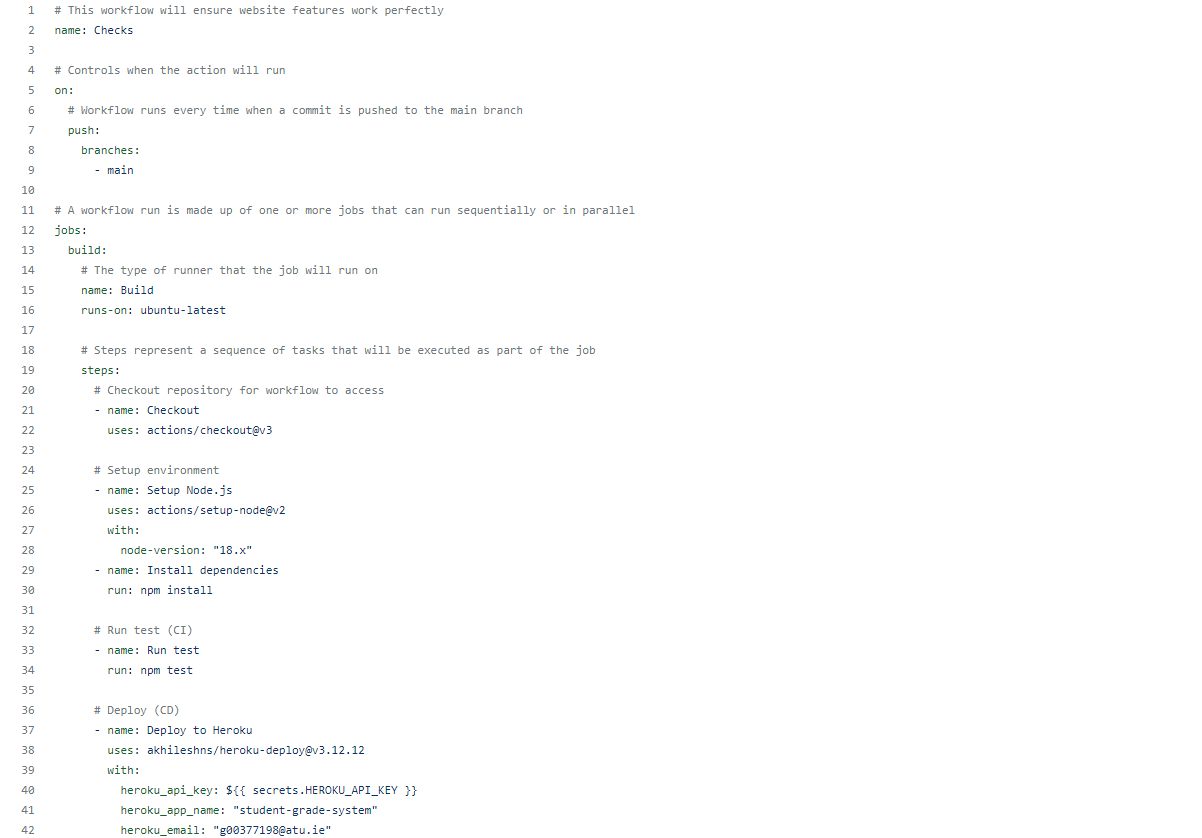
\includegraphics[width=1.5\textwidth]{images/full-workflow.png}
    \caption{GitHub Actions Workflow}
    \label{image:full-workflow}
\end{figure}

Overall, this workflow ensures that the website's features work perfectly by building, testing, and deploying the system automatically in response to changes in the main branch.

The \texttt{npm test} in the workflow file runs the tests automatically from the directory. The test file was design using Supertest and Jest to test out CRUD API with a test suite with five test cases:

\begin{enumerate}
  \item Able to CREATE a new student information to database
  \item Able to READ all student information from database
  \item Able to READ a specific student information from the database for update
  \item Able to UPDATE a student information
  \item Able to DELETE a student information
\end{enumerate}

The code snippet from Figure~\ref{image:test-create} below tests the functionality of a create functionality, specifically, the \texttt{createGrade} function that creates a new student record. It sends a HTTP POST request to the \textit{/createGrade} endpoint with test data and expects a response status code of 200 and a response message of 'Student Grade Added'. It stores the ID of the newly created student record in a variable called \texttt{testId} to test out other functionalities. This test case ensures that the \texttt{createGrade} function is able to create new student records without errors.

\begin{figure}[h!]
    \centering
    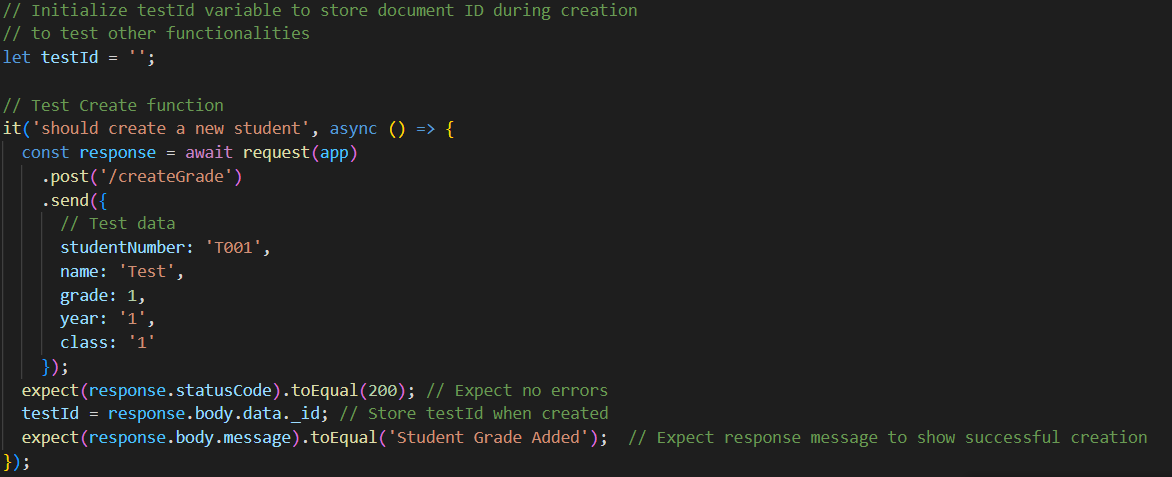
\includegraphics[width=0.9\textwidth]{images/test-create.png}
    \caption{Test Create Functionality}
    \label{image:test-create}
\end{figure}

After ensuring the application is working as expected by running the test suite, the workflow uses Heroku, a Platform as a Service (PaaS), to deploy the application. It is vital to note that \textit{Procfile} is included in the directory as it specifies the commands that are executed by the application on startup, and the server will be started up in this context. After running the server side, the Heroku post-build is used to run the build file to show the frontend. Figure~\ref{image:heroku-build} below shows that \texttt{heroku-postbuild} is added under the script in package-json.

\begin{figure}[h!]
    \centering
    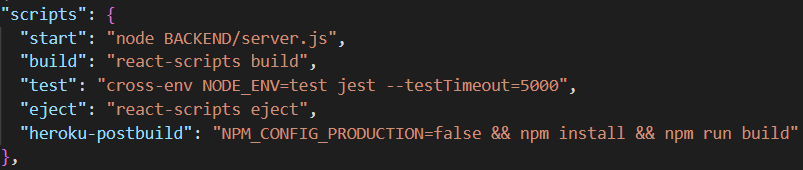
\includegraphics[width=0.9\textwidth]{images/heroku-build.png}
    \caption{Code Snippet from package.json to show heroku-postbuild}
    \label{image:heroku-build}
\end{figure}

\section{MongoDB Database Design}

For this project, there is a collection in the database called \textit{grades} with the following structure:

\begin{table}[ht]
    \centering
    \begin{tabular}{|p{3.5cm}||p{3cm}||p{5.5cm}|}
    \hline
    \textbf{Field} & \textbf{Datatype} & \textbf{Special Conditions} \\
    \hline \hline
    \textunderscore id  & ObjectId & Auto-generated by database \\
    \hline
    studentNumber  & String & Required \\
    \hline
    name & String & Required \\
    \hline
    grade & String & Required \\
    \hline
    year & String & Required \\
    \hline
    class & String & Required \\
    \hline
    \end{tabular}
    \linebreak
        \caption{MongoDB Structure}
        \label{tab:mongodbstruc}
\end{table}

The \textit{\textunderscore id} that is generated automatically by MongoDB is used to get specific document from the database while the rest is just the data for the application which is required as stated.

\section{MERN Stack}
As discussed previously in methodology with reference to Figure~\ref{appendix:mern} in Appendix~\ref{appendix:mern}, The database used for the system is MongoDB, the frontend or the webpage is developed using React.js and the backend or the server is built using Node.js with Express.js framework. The CRUD functionalities that are implemented in the student grade system for this project are as follows:

\begin{itemize}
\item Create: Add a student with grades and other information.
\item Read: Get all students' information and filter certain categories of students.
\item Update: Update student grades and/or information.
\item Delete: Delete a student.
\end{itemize}

The above functionalities are designed as APIs in the backend with the frontend used for interaction and the database utilized for managing the data.
